

\documentclass[a4paper, 11pt]{article} 



\usepackage{graphicx} 

\usepackage[parfill]{parskip} % Activate to begin paragraphs with an empty line rather than an indent

%%% PACKAGES
\usepackage{booktabs} % for much better looking tables
\usepackage{threeparttable} % three-part-table
\usepackage{array} % for better arrays (eg matrices) in maths
\usepackage{paralist} % very flexible & customisable lists (eg. enumerate/itemize, etc.)
\usepackage{verbatim} % adds environment for commenting out blocks of text & for better verbatim
\usepackage[utf8, latin1]{inputenc} 
\usepackage{subfig} % make it possible to include more than one captioned figure/table in a single float
\usepackage{floatrow} % add notes below figure
\usepackage{lscape} %turn landscape
\usepackage{multirow}
\usepackage{amsmath} %math formatting
\usepackage{amssymb} %math formatting
\usepackage{tabulary} %table formatting
\usepackage{xcolor} %text color for annotations
\usepackage[colorlinks, citecolor=blue]{hyperref} % makes for easy anchor tags in document
\usepackage{ragged2e}

\renewcommand{\thesection}{\Alph{section}.}

\title{EDLD 650: Data Analysis and Replication Exercise (DARE) 1
Answer Key}

\author{David D. Liebowitz}
\date{Jan. 26, 2024} 

\begin{document}
\maketitle

\section{Data Management Tasks (1 point)}
\begin{enumerate}
	\item[A1.] See model code and comments.
	\item[A2.] See model code and comments. Note that you should assign states that never implemented evaluation a common value (typically -1 but it could be anything actually). You should also censor the top and bottom values at 6 years prior and 3 years post evaluation implementation following Liebowitz and co-authors.
\end{enumerate}

\section{Understanding the Data and Descriptive Statistics (3 points)}
\begin{enumerate}
	\item[B1.] There are a total of 516 state-year observations in the data, but 46 state-year observations are missing values for all outcomes and covariates. These represent states in which no schools participated in tracking the implementation of schoolwide PBIS. While this missingness does not necessarily bias our findings, it limits their external generalizability. We will need to either (a) be very clear in the interpretation of our results as being specific to the population to which we are inferencing (see B3); (b) make a convincing argument about why our results might generalize beyond this population; or (c) both. We are less concerned about demographic or other covariate missingness, as we have tools to impute those values and test whether or not our imputation decisions (to the extremes) influence our final estimates. 
	
	\item [B2.] In \autoref{fig:outcome}, we present histograms that describe the range of all four outcome categories of Office Disciplinary Referalls (ODRs). We observe that their distributions are roughly symmetric. However all four outcome variables are positively skewed; in some states and some years, the average rate at which students are removed from class far exceeds five referrals per 500 students per day. Distributions with large clusters near zero and several outlying values several orders of magnitude higher are candidates for log transformations or estimation via Poisson regression. However, such transformations or alternative modeling structures can make interpretation of results more difficult. As the tail of the distribution is relatively thin and only one order of magnitude larger than the mean, we preserve the original scale in our analyses.

	We would want to first inspect those higher values of our outcome variables to ensure they are not errors. If we conclude that those higher values do not represent any coding or reporting errors (as we do), we would be interested in determining whether these extreme values represent states for which only a small number of schools are present in our sample or data points early in the sample in which behavioral systems may have been weaker in many of the schools. The second instance might be informative to understanding secular trends in our data. We may also assess whether schools in states with higher ODR values before PBIS implementation were systematically different from those with lower initial ODR values, and if their exclusion from the analysis led to any different substantive conclusion. 

\begin{figure} [!htbp]
\begin{center}
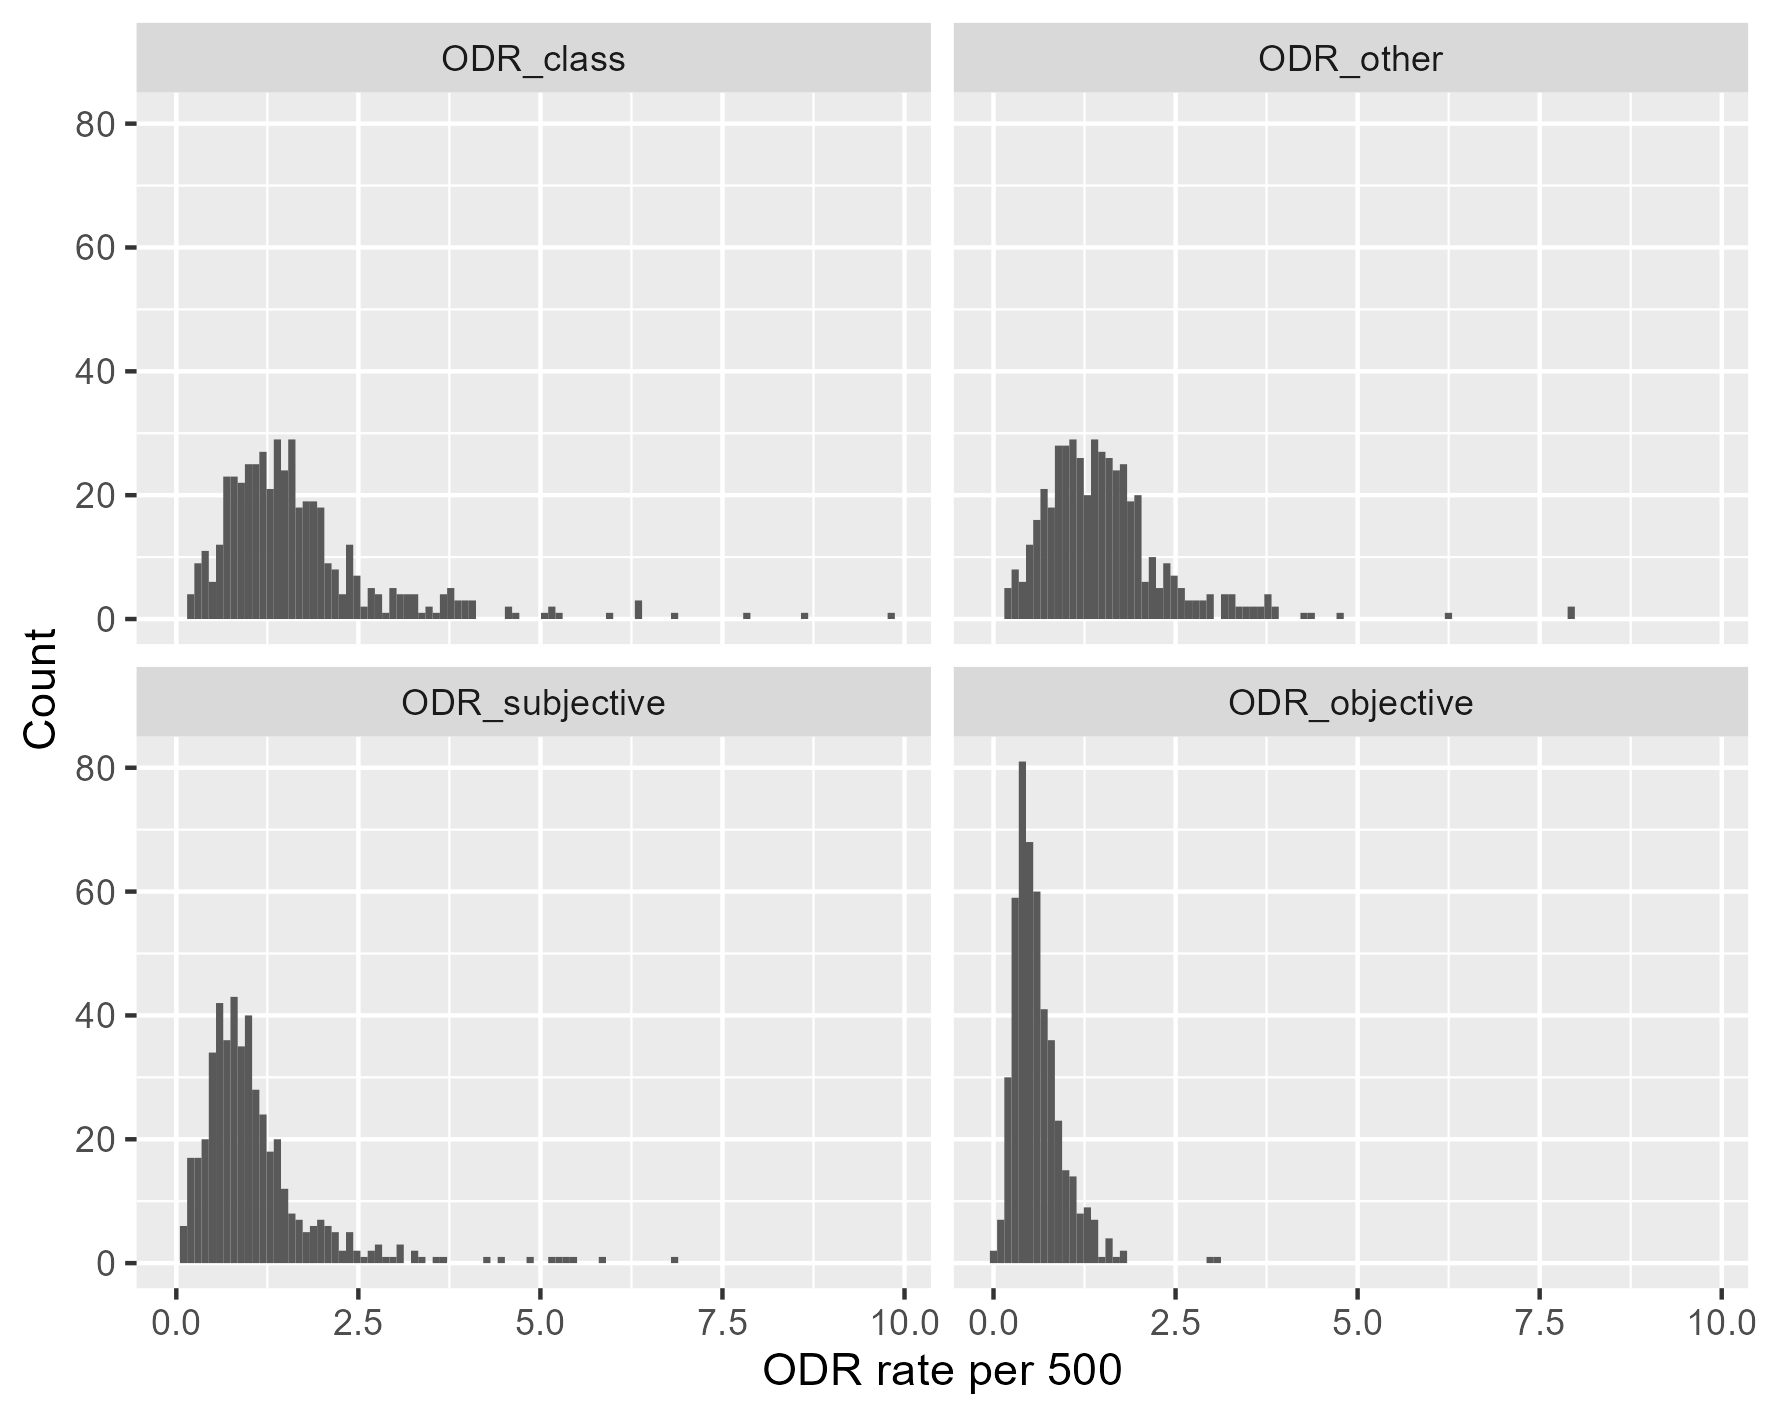
\includegraphics[scale=0.8]{figures/odr_hist.png}
\caption{Rates of Office Disciplinary Referrals (ODRs) by state-years}
 \label{fig:outcome}
\end{center}
\end{figure}

	\item[B3.] Our sample consists of states in which there exist schools that have attempted to implement PBIS, use the SWIS data management system, and have consented to have their data used for research purposes. In these states, there exist at least some schools (minimally one school) which have data on all four categories of Office Disciplinary Referrals. This is the broader population to which we draw our inferences.
	
	In \autoref{tab:descriptives}, we present descriptive statistics on our analytic sample of 470 state-year observations. The average state-year observation represents a student enrollment of just less than 22,000 students, and our dataset represents over 880,000 students per year over the 12-year sample. Demographic and outcome statistics are weighted by total state-year enrollment. 55 percent of students in states represented in our sample are, on average, from low-income families. In our analytic sample, the average per-day number of referrals from classroom settings is 1.39 per 500 students and the average per-day number of referrals from all other settings is 1.33 referrals per 500 students. Analogously, the average per-day number of referrals for subjective reasons is 0.87 per 500 students and 0.53 per 500 students for objective reasons. In our sample, of the 341 state-year observations for which we have available implementation fidelity data, 72 percent successfully implement PBIS in a given year. The mean demographic characteristics in our data are broadly similar to Liebowitz, Porter and Bragg (2022). However, their standard deviations are much narrower, given that values are summarized at the state (rather than grade-within-school) level, and we calculate standard deviations within state-year. As there is less overall variation in these covariates, this implies that they will absorb less of the outcome variation; thus, having a more modest impact on our statistical power.
	
	In our sample, states have lower mean rates of disciplinary referrals (ODRs) and their standard deviations are much lower than in Liebowitz and co authors. As a result, we will again have less power and the precision of our estimates will be lower. This means the confidence intervals around our estimates, as expressed in standard deviations of our outcomes, will be larger. If we find similar results as the original paper, we may be able to confidently rule out only very large effect sizes.


% Table created by stargazer v.5.2.2 by Marek Hlavac, Harvard University. E-mail: hlavac at fas.harvard.edu
% Date and time: Wed, Jan 05, 2022 - 1:00:32 PM
\begin{table}[!htbp] \centering 
  \caption{Descriptive Statistics} 
  \label{} 
\begin{tabular}{@{\extracolsep{5pt}}lccc} 
\\[-1.8ex]\hline 
\hline \\[-1.8ex] 
Statistic & \multicolumn{1}{c}{N} & \multicolumn{1}{c}{Mean} & \multicolumn{1}{c}{St. Dev.} \\ 
\hline \\[-1.8ex] 
Mean State-Year Enrollment & 470 & 21,897 & 4,622 \\ 
Mean Yearly Enrollment & 470 & 881,631 & 232,717 \\ 
Pct. low-income & 470 & 0.55 & 0.05 \\ 
Pct. American Indian/Native AK & 470 & 0.01 & 0.001 \\ 
Pct. Asian/Pacific-Islander & 470 & 0.05 & 0.01 \\ 
Pct. Black & 470 & 0.13 & 0.02 \\ 
Pct. White Non-Hispanic & 470 & 0.55 & 0.02 \\ 
Pct. Hispanic & 470 & 0.19 & 0.05 \\ 
Pct. States by year Implementing PBIS & 341 & 0.72 & 0.45 \\ 
Daily Referalls per 500 students - Classroom & 470 & 1.39 & 0.14 \\ 
Daily Referalls per 500 students - Other & 470 & 1.33 & 0.13 \\ 
Daily Referalls per 500 students - Subjective & 470 & 0.87 & 0.10 \\ 
Daily Referalls per 500 students - Objective & 470 & 0.53 & 0.05 \\ 
\hline \\[-1.8ex] 
\multicolumn{4}{l}{Notes: This table presents state-year means and standard deviations from 2006-2018.} \\ 
\end{tabular} 
\end{table} 


	\item[ B4.] \textbf{\textit{Optional}} In \autoref{fig:means}, we observe that there was a gradual downward \textit{secular trend} in the number of disciplinary referrals as states approached and then passed teacher evaluation reform. This secular trend does not bias our estimates as our year fixed effects will adjust for these differing values by year. However, we are interested in looking for any discontinuities around the enactment of the teacher evaluation policy reforms. 
	
	\begin{figure} [!htbp]
		\begin{center}
			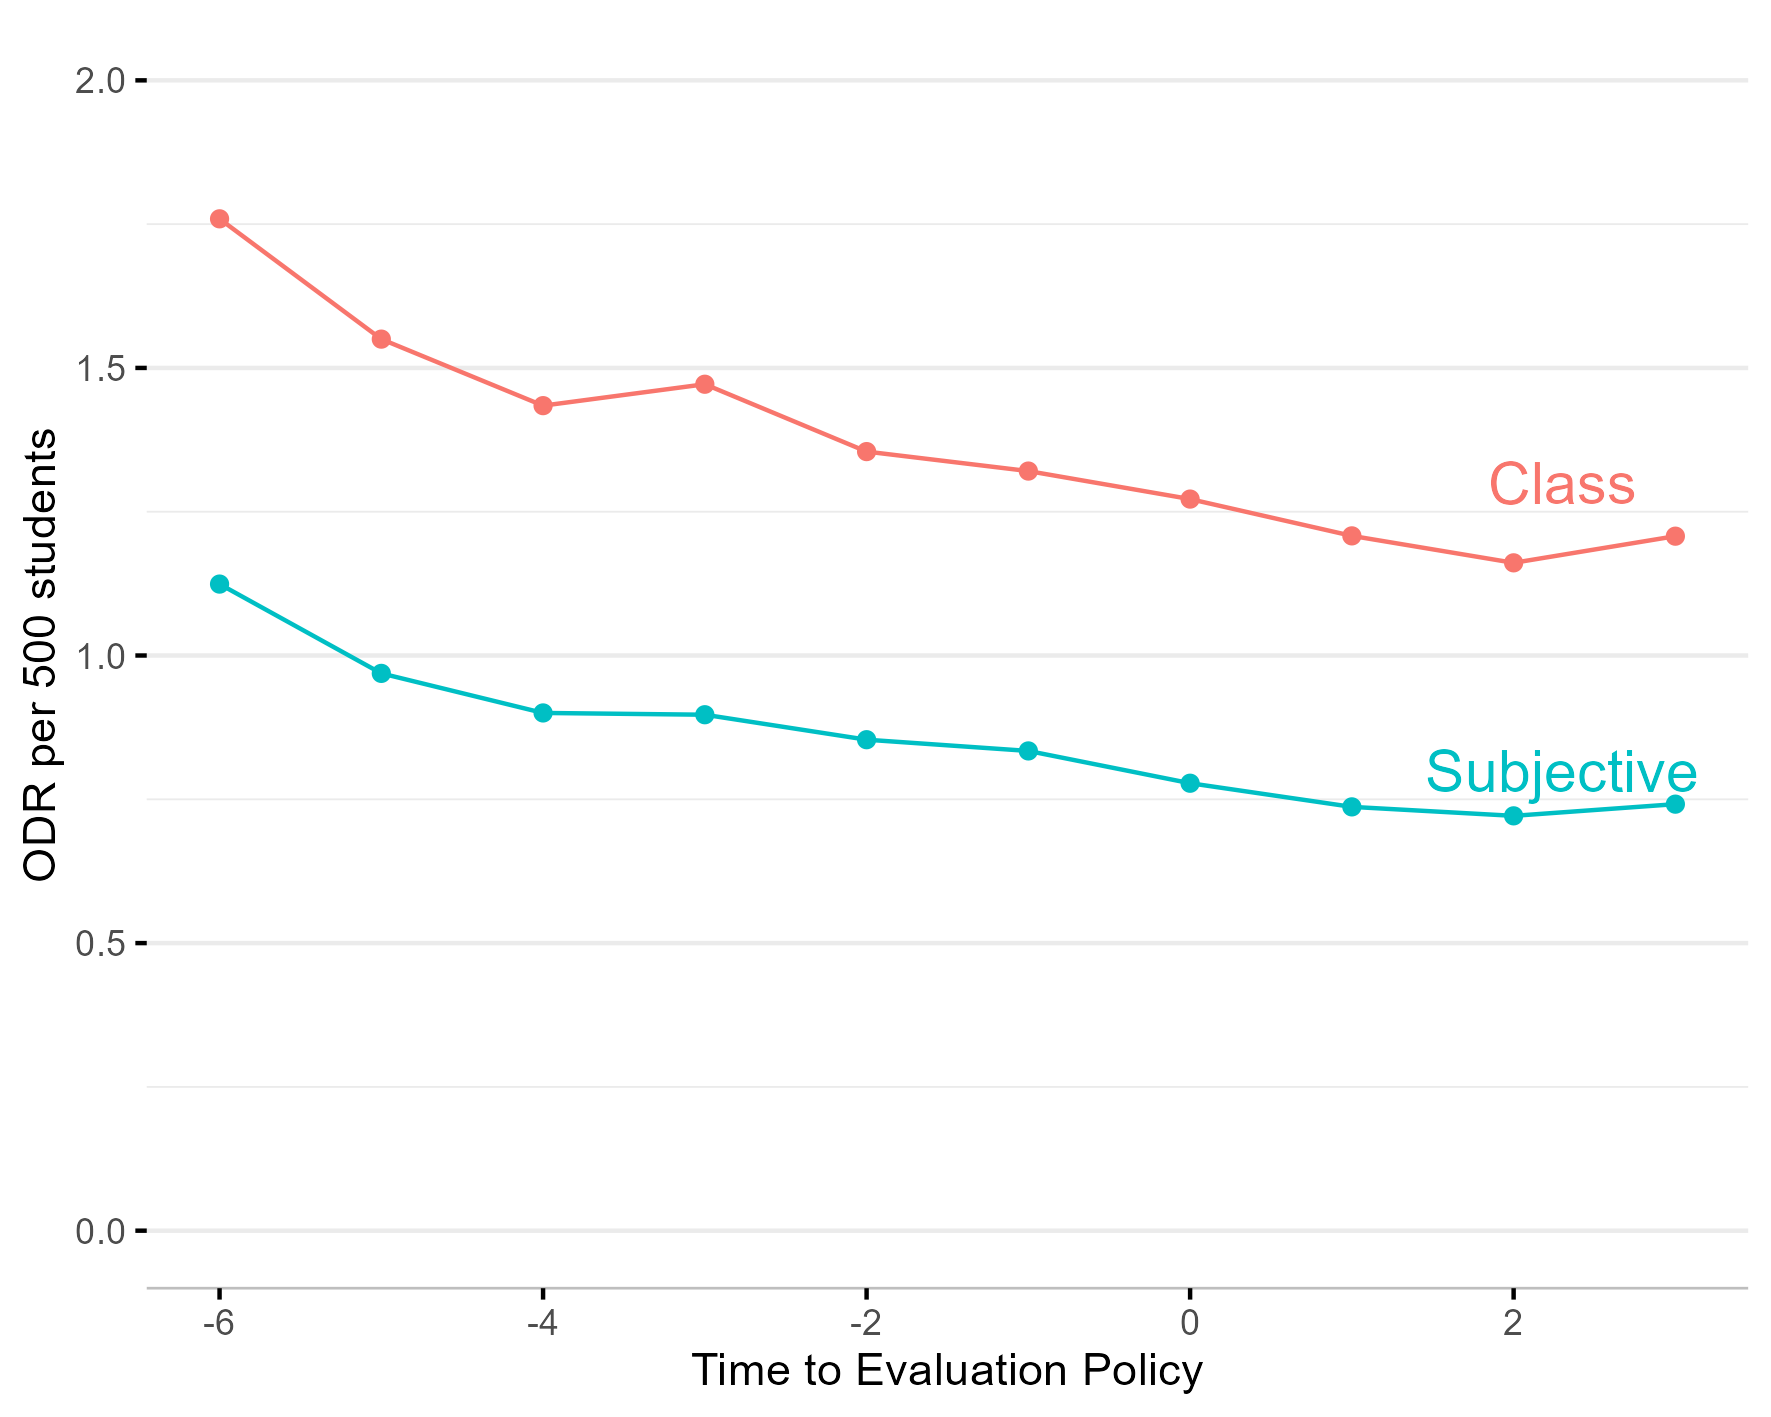
\includegraphics[scale=0.8]{figures/averages.png}
			\caption{Average office disciplinary referral rates, relative to states' adoption of higher-stakes evaluation policies}
			 \label{fig:means}
		\end{center}
	\end{figure}

These raw averages show us that, at first glance, there are no obvious jumps in the rate of referrals coincidental with the policy change. However, we recognize that more advanced difference-in-difference estimation strategies that attempt to account for secular trends may generate different results. 

States that never implemented changes to their teacher evaluation laws never experience a condition in which they are a given number of years prior to or after evaluation policy. If we included these states, the way we currently have them coded, their ODR rate values would all be contributing to the omitted category (-1). Doing so would likely change the observed ODR rate at -1. Thus, the value at -1 would no longer represent that in which we are most interested: the rate of ODRs in states that ultimately implement the policy change in the year prior to implementation. 

\end{enumerate}


\section{Replication and Extension (6 points)}


\begin{enumerate}
	\item[C1.] We fit the following difference-in-differences model to test the effect of the implementation of higher-stakes teacher evaluation policy on the rates of office disciplinary referrals (ODRs):

\begin{equation} \label{eq:1}
ODR_{st}=\beta_{1} EVAL_{st}+\left(\mathbf{X}_{st}\right) \theta+\Gamma_{s}+\Pi_{t}+\mu_{st} 
\end{equation}

where $ODR_{st}$ represents the per-500-student per-day rate of Office Disciplinary Referrals for each state-year observation regressed on an indicator, $EVAL_{st}$, that takes on a value of 1 if state ($s$) has high-stakes teacher evaluation policy implemented in year ($t$). $\mathbf{X}_{\mathrm{st}}$ is a parsimonious vector of plausibly exogenous school characteristic adjustments to capture state-specific characteristics and improve the precision of our estimates. $\Gamma_s$ and $\Pi_t$ are state- and year-fixed effects, respectively. We cluster standard errors at the state-by-year level, which is the unit of treatment.

We extend our analysis by relaxing the assumption of the standard difference-in-differences model of time-invariant treatment by allowing treatment effects to vary post evaluation reform:

\begin{equation} \label{eq:2}
\begin{aligned} 
ODR_{st}= & \beta_{1} EVAL_{st}+\beta_{2} (EVAL \times YEAR)_{st}+\beta_{2} YEAR_{st}+ \\
& \left(\mathbf{X}_{\mathrm{st}}\right) \theta+\Gamma_{s}+\Pi_{t}+v_{st}
\end{aligned}
\end{equation}

We include a linear time trend ($YEAR_{st}$), which is centered at the year in which the state implemented high-stakes teacher evaluation policy. The main effect of $YEAR_{st}$ serves as a test of the parallel trends assumption. We model the interaction ($EVAL\times YEAR_{st}$) which allows time trends in treated states to vary post-reform. We fit the model first with classroom ODRs as the outcome of interest, then classroom subjective ODRs. All other terms are defined as above.

As we document in \autoref{tab:mainDD}, we find no evidence that the implementation of higher-stakes teacher evaluation changed the rate of disciplinary referrals, for either classroom or classroom-subjective ODRs. Models 1 and 4 include only the main policy predictor in addition to the state- and year-fixed effects. While the signs are negative, the magnitudes are small and statistically indistinguishable from zero. In rejecting our null hypothesis, we conclude in both cases that implementing teacher evaluation reform has no effect on office disciplinary referrals, on average in the population. 

The results hold when we include statistical adjustments for student demographics in Models 2 and 4. Models 3 and 6, which allow the effects to differ post-reform are also indistinguishable from zero. In addition, the coefficients on the time-trend ($YEAR_{st}$) are also indistinguishable from zero, providing suggestive evidence that our un- or not-yet-treated states were on parallel prior trends.

\begin{table}

\caption{The effect of teacher evaluation reforms on Office Disciplinary Referrals, by location and subjectivity \label{tab:mainDD}}
\centering
\begin{threeparttable}
\begin{tabular}[t]{lcccccc}
\toprule
   & \multicolumn{3}{c}{Class} & \multicolumn{3}{c}{Subjective}\\
  & (1) & (2) & (3) & (4) & (5) & (6)\\
\midrule
Implement evaluation & -0.060 & -0.075 & -0.065 & -0.046 & -0.049 & -0.040\\
 & (0.058) & (0.082) & (0.074) & (0.044) & (0.058) & (0.048)\\
Eval x Relative-Year &  &  & 0.021 &  &  & 0.014\\
 &  &  & (0.032) &  &  & (0.020)\\
Pre-trend &  &  & -0.012 &  &  & -0.009\\
 &  &  & (0.035) &  &  & (0.025)\\
\midrule
Covariates? &  & X & X &  & X & X\\
Num.Obs. & 470 & 470 & 470 & 470 & 470 & 470\\
R2 & 0.825 & 0.836 & 0.836 & 0.816 & 0.829 & 0.830\\
\bottomrule
\end{tabular}
\begin{tablenotes}
\item Notes: $^{+}p<0.1, ^{*}p<0.05, ^{**}p<0.01, ^{***}p<0.001$. The table displays coefficients from Equations 1 and 2 and state-by-year-clustered standard errors in parentheses. All models include fixed effects for year and state and are weighted by state enrollment. Models 2-3 and 5-6 adjust for the proportion of FRPL-eligible students and the proportion of students of different ethnoracial backgrounds.
\end{tablenotes}
\end{threeparttable}
\end{table}


	\item[C2.] One key assumption of our identification strategy is that there are no simultaneous policy shocks or secular trends that bias the estimates. It is reasonable to believe that policy changes altering teachers' authority to remove students from the classroom or schools' ability to suspend students, might affect the ODR rate. To test this possibility, we fit a series of models to test whether any of these three policy indicators predict changes in rates of office referrals. As seen in \autoref{tab:alt}, we find no evidence that simultaneous changes in teacher authority to remove students from class or schools' ability to suspend students significantly affected the ODR rate, either estimated independently or in conjunction with the effect of evaluation implementation. 


\begin{table}[!htbp]
   \caption{\label{tab:alt} Alternative policy robustness checks}
   \bigskip
   \centering
   \begin{tabular}{lcccccc}
      \hline \hline \\[-1.8ex]
       & \multicolumn{3}{c}{Class} & \multicolumn{3}{c}{Subjective}\\
                           & (1)           & (2)           & (3)           & (4)           & (5)           & (6)\\  
      \midrule 
      Class remove reform  & 0.103         &               & 0.093         & 0.073         &               & 0.078\\   
                           & (0.081)       &               & (0.081)       & (0.052)       &               & (0.056)\\   
      Limit suspension     &               & 0.068         & 0.064         &               & 0.019         & 0.011\\   
                           &               & (0.052)       & (0.053)       &               & (0.036)       & (0.038)\\   
      Implement Evaluation &               &               & -0.093        &               &               & -0.057\\   
                           &               &               & (0.048)       &               &               & (0.034)\\   
       \midrule
      R$^2$                & 0.836         & 0.835         & 0.837         & 0.829         & 0.829         & 0.830\\  
      Observations         & 470           & 470           & 470           & 470           & 470           & 470\\  
       \midrule
      State fixed effects  & $\checkmark$  & $\checkmark$  & $\checkmark$  & $\checkmark$  & $\checkmark$  & $\checkmark$\\   
      Year fixed effects   & $\checkmark$  & $\checkmark$  & $\checkmark$  & $\checkmark$  & $\checkmark$  & $\checkmark$\\   
      \hline \hline \\[-1.8ex]
   \end{tabular}
   
   \par \justifying 
   \small \textit{Notes}: $^{*}p<0.05, ^{**}p<0.01, ^{***}p<0.001$. Cells report coefficients and state-by-year clustered standard errors in parentheses. All models include fixed effects for year and state, are weighted by state enrollment, and adjust for the proportion of FRPL-eligible students and the proportion of students of different ethnoracial backgrounds.
\end{table}




Another key assumption is that the comparison group identified serves as a valid counterfactual to the treated group. One concern may be that states which choose to implement higher-stakes teacher evaluation policies have selected into treatment and are therefore driven to do so by endogenous differences from states that were not. As a check, we restrict our sample to only states that ever implemented evaluation, thereby using only the not-yet-treated states as the comparison group and addressing concerns that there may be unobserved differences between never-treated and eventually-treated states. As we demonstrate in \autoref{tab:robust}, Models 1 and 3, the estimates are statistically indistinguishable from zero. 

We may also be concerned that our difference-in-difference results are driven by events substantially removed from policy enactment, particularly when we observe these time periods for only some units. Given the start and end periods of our data, the maximal years pre- and post-teacher evaluation reform that we can see for all observations is 5 years pre- and 1 year after the initial policy implementation. Models 2 and 4 in \autoref{tab:robust} restrict our sample to state-year observations during this time frame. Again, we fail to reject the null hypothesis.


\begin{table}[!htbp]
   \caption{\label{tab:robust} Treated-only and balanced-panel robustness checks}
   \bigskip
   \centering
   \begin{tabular}{lcccc}
       \hline \hline \\[-1.8ex]
       & \multicolumn{2}{c}{Class} & \multicolumn{2}{c}{Subjective}\\
                           & (1)           & (2)           & (3)           & (4)\\  
      \midrule 
      Implement Evaluation & -0.074        & -0.081        & -0.045        & -0.047\\   
                           & (0.050)       & (0.047)       & (0.035)       & (0.032)\\   
       \midrule
      R$^2$                & 0.821         & 0.884         & 0.802         & 0.887\\  
      Observations         & 399           & 326           & 399           & 326\\  
       \midrule
      State fixed effects  & $\checkmark$  & $\checkmark$  & $\checkmark$  & $\checkmark$\\   
      Year fixed effects   & $\checkmark$  & $\checkmark$  & $\checkmark$  & $\checkmark$\\   
       \hline \hline \\[-1.8ex]
   \end{tabular}
   
   \par \justifying
   \small \textit{Notes:} $^{*}p<0.05, ^{**}p<0.01, ^{***}p<0.001$. Cells report coefficients and state-by-year clustered standard errors in parentheses. Models 1 and 3 are limited to states that ever implemented teacher evaluation reforms. Models 2 and 4 are estimated in balanced panels, restricted to state-year observations 5-years before and 1-year after evaluation reform. All models include fixed effects for year and state, are weighted by state enrollment, and adjust for the proportion of FRPL-eligible students and the proportion of students of different ethnoracial backgrounds.
\end{table}





	\item[C3.] Our main findings are that high-stakes teacher evaluation has no causal effect on the overall rate of classroom or subjective-classroom ODRs. However, our estimates of these null effects are quite imprecise. We cannot rule out effects smaller than a decrease of approximately 1.25 standard deviations (\textit{SDs}) or an increase around 0.5 \textit{SDs} for classroom and subjective-classroom referrals. Our results are robust to alternative policy shocks and sample specifications. We find no evidence of a moderating effect when schools improve their implementation of a widely-used behavioral improvement strategy known as Positive Behavioral Interventions and Supports (PBIS). 
	
	\item[C4.]  \textbf{\textit{Optional }} In addition to the above parametric difference-in-difference estimates, we also fit a fully flexible event-study model as follows:
	\makeatletter
	\@hyper@itemfalse
	\makeatother
\begin{equation} \label{eq:3}
\begin{aligned}
ODR_{st}=\sum_{r=-5}^{1} 1\left(t=t_{s}^{*}+r\right) \beta_{r}+\left(\mathrm{X}_{\mathrm{st}}\right) \theta+\Gamma_{s}+\Pi_{t}+\varepsilon_{st}
\end{aligned}
\end{equation}

The causal estimate of interest is the series of $\beta$s in \autoref{eq:3}, which capture the effect of the policy in each given year ($r$) on the ODR rate. All effects are measured in comparison to the year prior to policy change $(r = -1)$ and all states that never implement the policy change are assigned a value of $r = -1$. All other terms are defined as above. The event study allows us to model the estimated policy effects without the assumption of a functional form in the treatment effect. 

\autoref{fig:event} presents the results of the non-parametric DD graphically. In Panel A, we see a slight decrease in ODRs in the years after the policy implementation, but all estimates are statistically indistinguishable from zero and small in magnitude. When looking at the effect of the policy change on subjective ODRs, we see a similar trend, with small negative estimates statistically indistinguishable from zero. 

Compared to Liebowitz and co-authors, we do observe a slight downward trend in the rates of ODRs in the years prior to policy enactment, particularly for subjective ODRs. We might want to restrict our analytic sample in these estimates to drop observations five years prior to policy enactment as the trend appears relatively flat in subsequent years. However, none of these estimates are statistically distinct from zero, so we are relatively confident using the full set of available data.


\begin{figure}
\begin{center}
\subfloat[Classroom ODRs]{%
  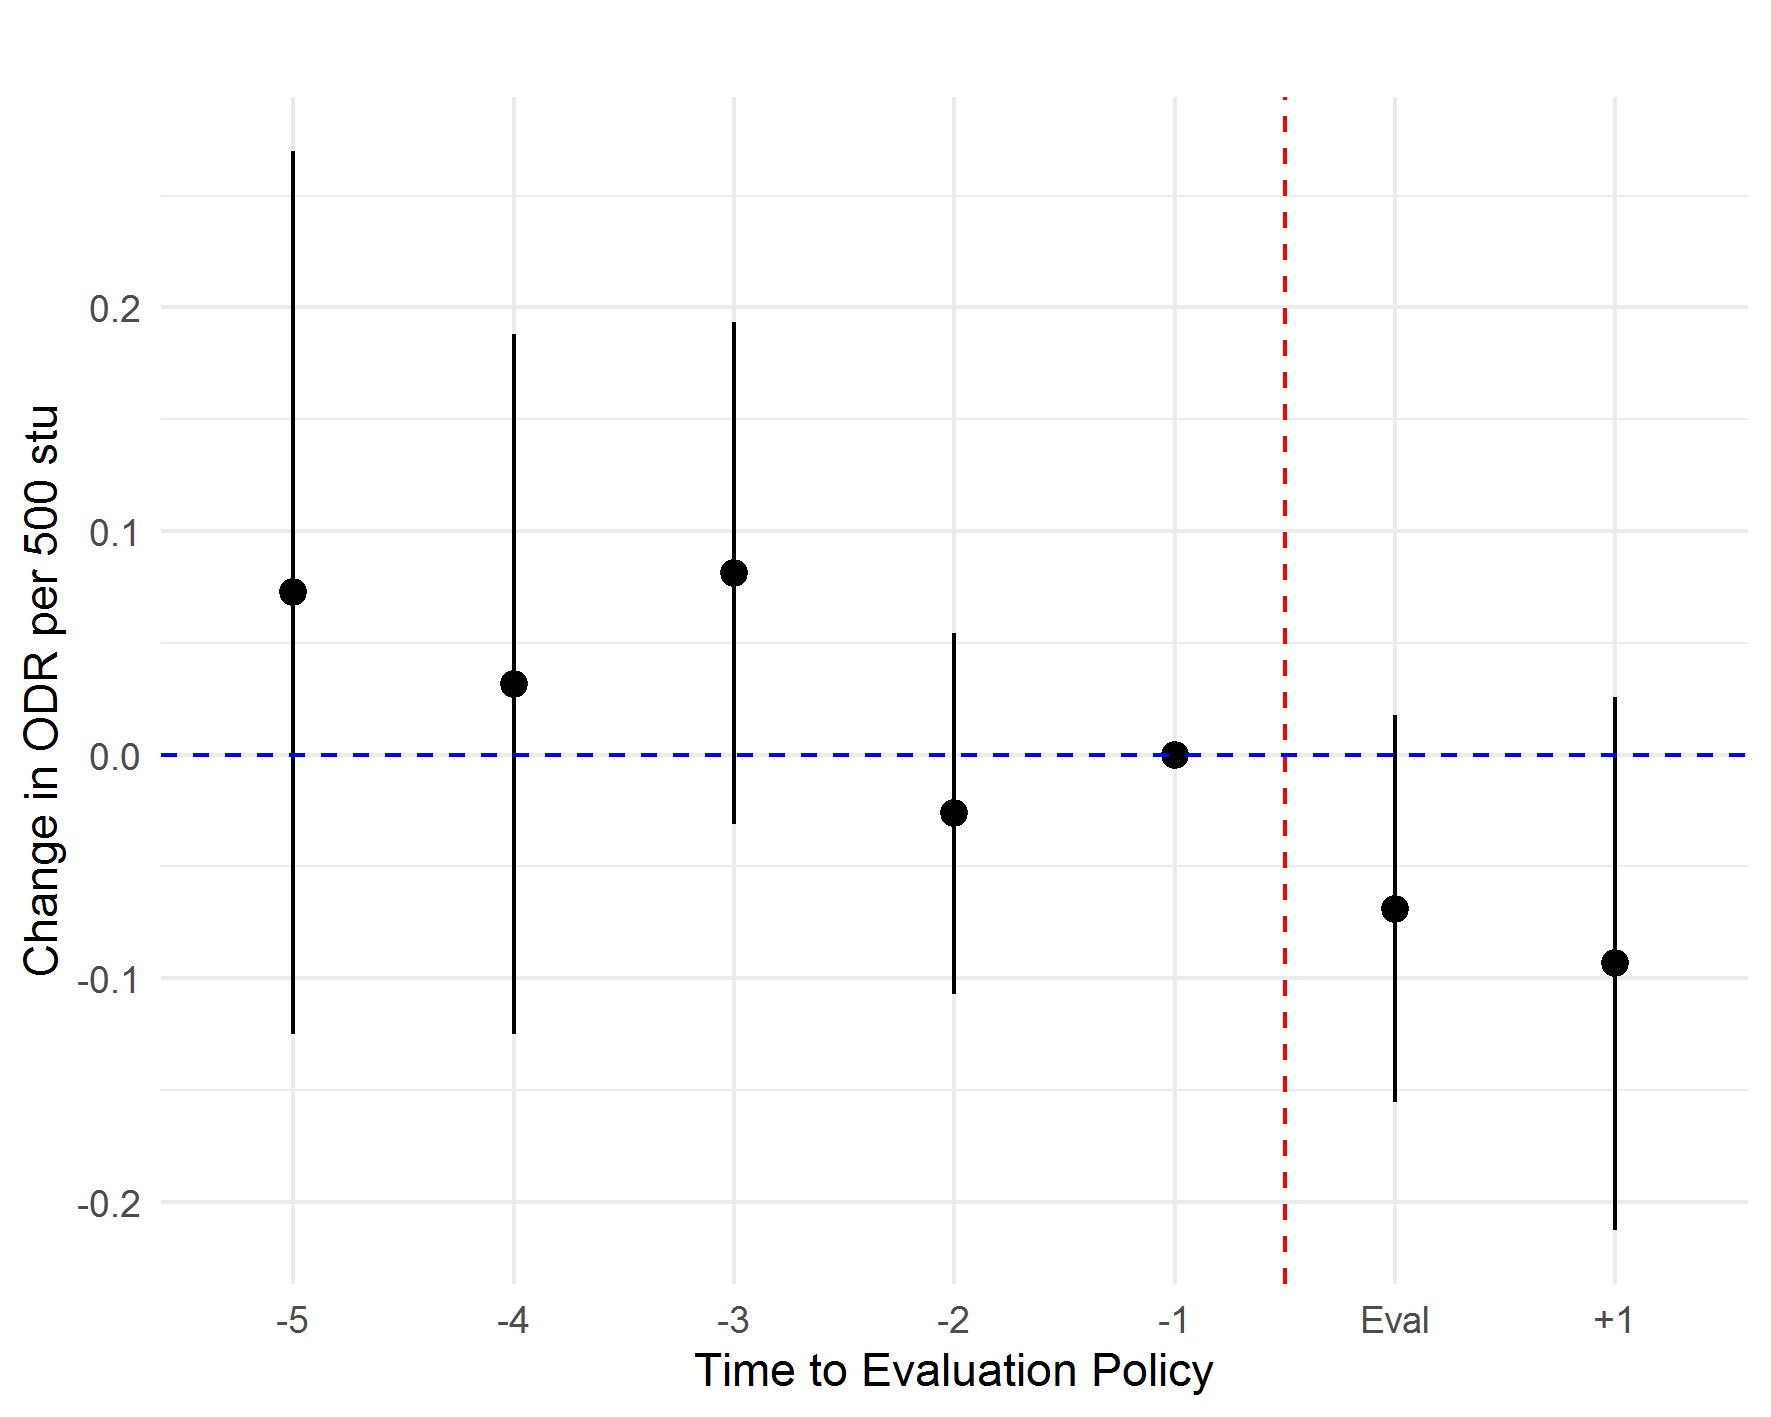
\includegraphics[scale=0.5]{figures/event_study_class.png}%
}

\subfloat[Classroom-Subjective ODRs]{%
  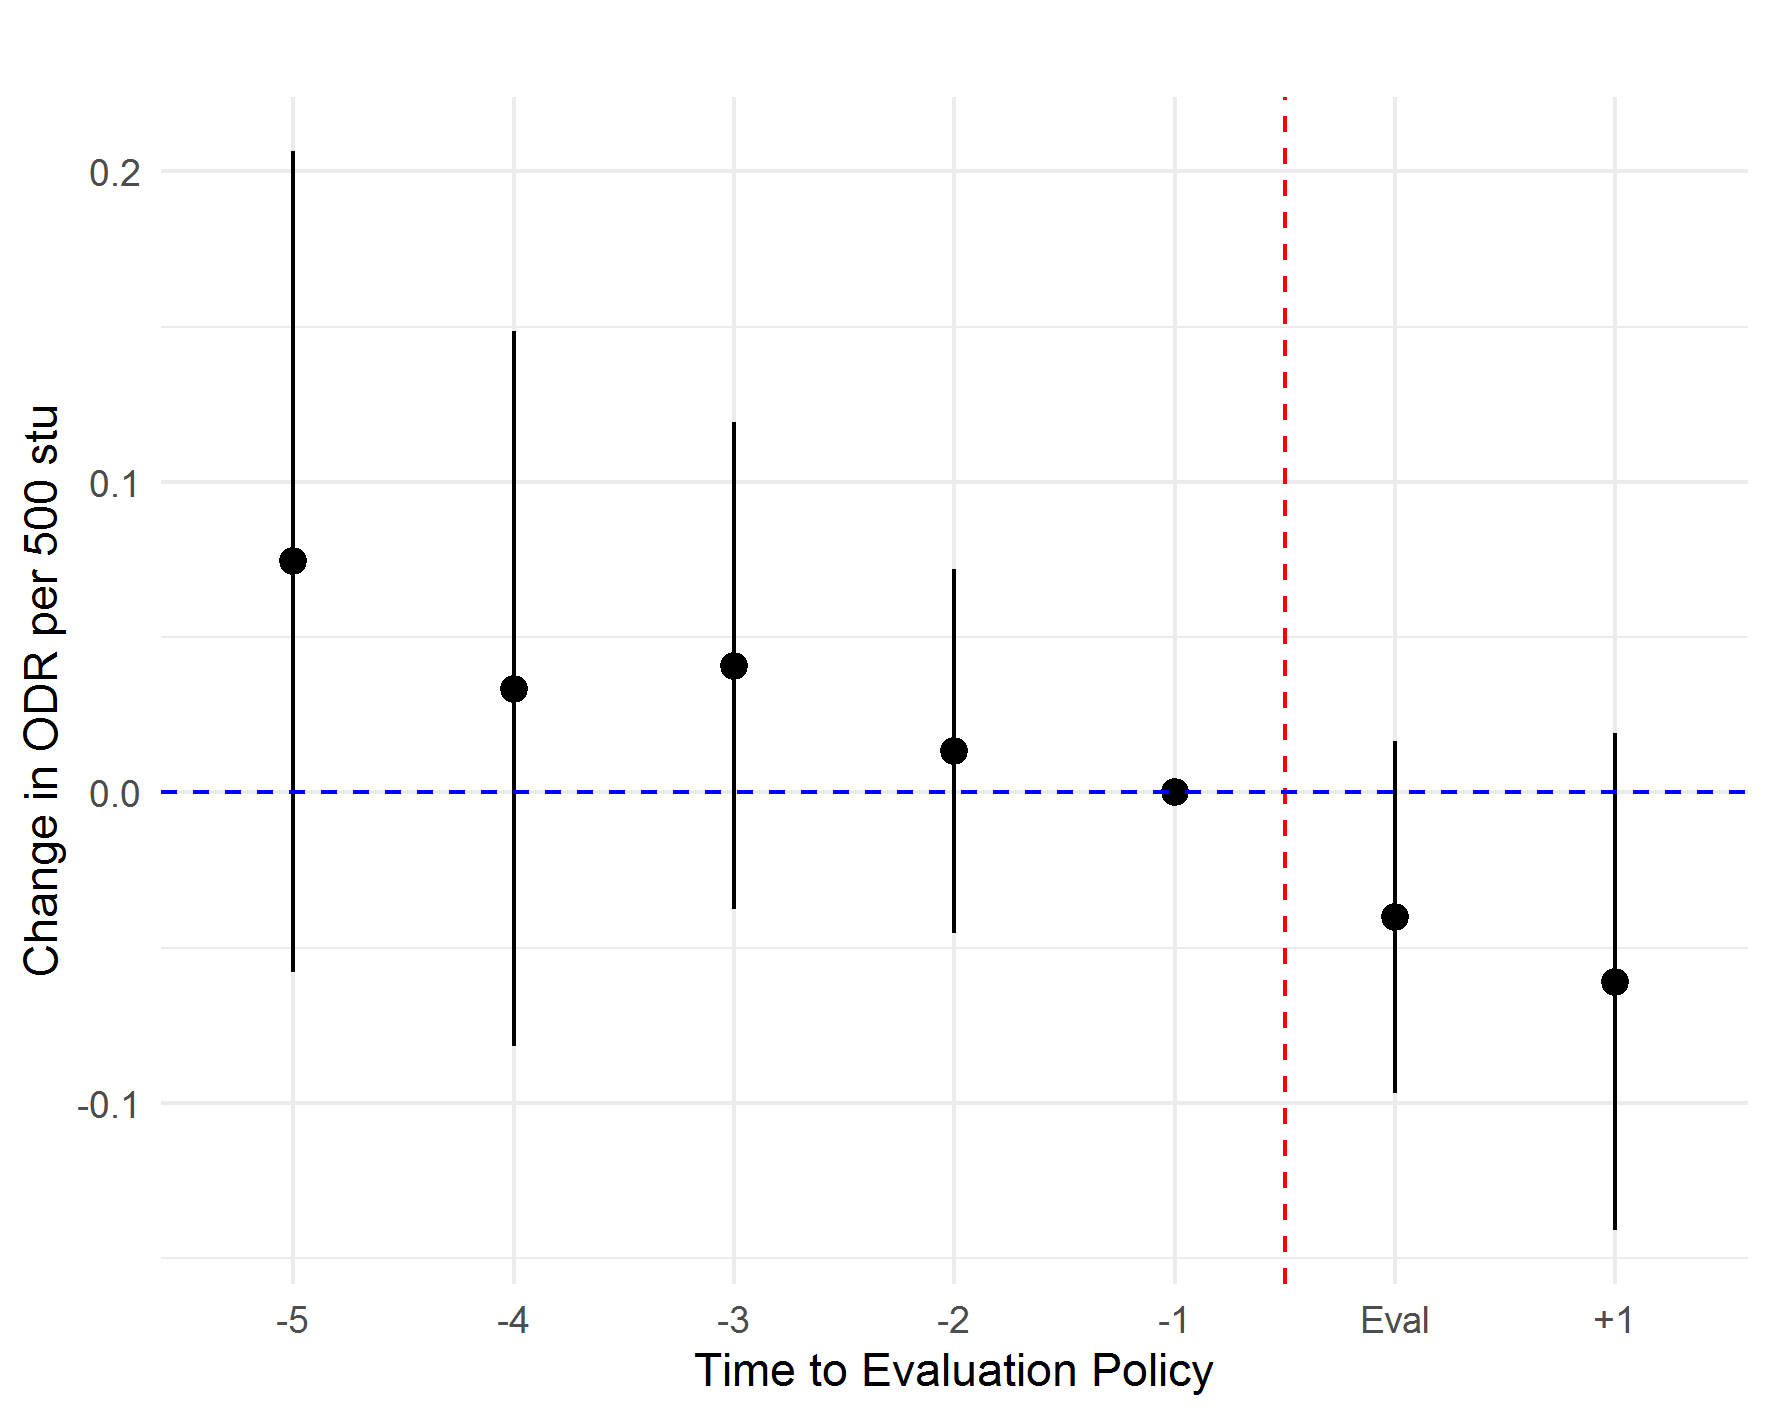
\includegraphics[scale=0.5]{figures/event_study_subjective.png}%
}

\caption{Event-study estimates of implementation of higher-stakes evaluation policy}
\label{fig:event}
\end{center}
	\floatfoot{\textit{Notes}: Point estimates and 95\% confidence intervals from \autoref{eq:3}.}
\end{figure}

	\item[C5.] \textbf{\textit{Optional }} We find no evidence that improvements in schools' implementation of Positive Behavioral Interventions and Supports (PBIS) practices serves to moderate the effects of accountability. We present results in \autoref{tab:pbis} of a series of estimates in the subset of state-year observations for which we have measures of PBIS implementation. As such measures are available in only 341 of our 470 state-year observations (73 percent), in Models 1 and 3 we first re-estimate the results from \autoref{tab:mainDD} and examine the main effect of evaluation implementation in this sub-sample of observations. For these states, the effects are even closer to zero. We then introduce the time-varying effect of PBIS implementation and its interaction with teacher evaluation (Models 2 and 5). We observe no moderating effects of successfully implementing PBIS on the effects of higher-stakes teacher evaluation. Finally, we relax our assumption of mean effects in Models 3 and 6. We find no evidence of post-evaluation implementation time trends. We observe no substantive differences with the results in the original paper.


\end{enumerate}

\begin{landscape}

\begin{table}[!htbp]
   \caption{\label{tab:pbis} Difference-in-differences estimates of moderating effects of successful PBIS implementation}
   \bigskip
   \centering
   \begin{tabular}{lcccccc}
      \hline \hline \\[-1.8ex]
       & \multicolumn{3}{c}{Class} & \multicolumn{3}{c}{Subjective}\\
                                              & (1)           & (2)           & (3)           & (4)           & (5)           & (6)\\  
      \midrule 
      Implement Evaluation                    & -0.032        & -0.084        & 0.039         & -0.030        & -0.051        & 0.043\\   
                                              & (0.043)       & (0.105)       & (0.148)       & (0.029)       & (0.070)       & (0.107)\\   
      Implement PBIS well                     &               & -0.037        & 0.174         &               & -0.010        & 0.163\\   
                                              &               & (0.075)       & (0.129)       &               & (0.052)       & (0.088)\\   
      Eval x PBIS                             &               & 0.023         & -0.160        &               & 0.011         & -0.122\\   
                                              &               & (0.104)       & (0.154)       &               & (0.067)       & (0.110)\\   
      Pre-trend                               &               &               & -0.034        &               &               & -0.031\\   
                                              &               &               & (0.030)       &               &               & (0.020)\\   
      Eval x Relative-Year                    &               &               & 0.077         &               &               & 0.069\\   
                                              &               &               & (0.067)       &               &               & (0.043)\\   
      Implement PBIS well $\times$ Pre-trend  &               &               & 0.060         &               &               & 0.049$^{*}$\\   
                                              &               &               & (0.030)       &               &               & (0.022)\\ 
      Eval X PBIS x Year                      &               &               & -0.065        &               &               & -0.064\\   
                                              &               &               & (0.076)       &               &               & (0.048)\\   
       \midrule
      R$^2$                                   & 0.870         & 0.877         & 0.880         & 0.864         & 0.872         & 0.876\\  
      Observations                            & 341           & 341           & 341           & 341           & 341           & 341\\  
       \midrule
      State fixed effects                     & $\checkmark$  & $\checkmark$  & $\checkmark$  & $\checkmark$  & $\checkmark$  & $\checkmark$\\   
      Year fixed effects                      & $\checkmark$  & $\checkmark$  & $\checkmark$  & $\checkmark$  & $\checkmark$  & $\checkmark$\\   
      \hline \hline \\[-1.8ex]
   \end{tabular}
   
   \par \justifying 
   \small \textit{Notes:} $^{*}p<0.05, ^{**}p<0.01, ^{***}p<0.001$. Cells report coefficients and state-by-year clustered standard errors in parentheses. Models 1 and 3 are limited to states that ever implemented teacher evaluation reforms. Models 2 and 4 are estimated in balanced panels, restricted to state-year observations 5-years before and 1-year after evaluation reform. All models include fixed effects for year and state, are weighted by state enrollment, and adjust for the proportion of FRPL-eligible students and the proportion of students of different ethnoracial backgrounds.
\end{table}



\end{landscape}


\end{document}
	